\documentclass{beamer}

\usetheme{Singapore}

\usepackage[latin1]{inputenc}
\usepackage[french]{babel}
\usepackage{graphicx}


\begin{document}

\title[�dition interactive de graphes]{�dition interactive de graphes\\ en g�om�trie hyperbolique}

\author{Benjamin Vadon}

\institute[TER 2006--2007]{Stage de TER 2006--2007 \\
effectu� sous la direction de Jean-Christophe Filli�tre \\
� l'INRIA Futurs, dans l'�quipe ProVal \\
Parc Club Universit�, 91893 ORSAY}

\begin{frame}
\titlepage
\end{frame}

\begin{frame}
  \frametitle{La visualisation de graphes}
  \begin{itemize}
  \item Un probl�me complexe
  \item De nombreux algorithmes, mais aucune solution g�n�rale 
  \item Une approche diff�rente 
    \begin{itemize}
    \item A. Miquel, \emph{Affichage g�n�rique d'arbres � l'aide de la g�om�trie hyperbolique} (JFLA 2000)
    \end{itemize}
  \end{itemize}
\end{frame}

\begin{frame}
  \frametitle{Visualisation d'arbre en g�om�trie hyperbolique}
  \begin{figure}
    \begin{center}
      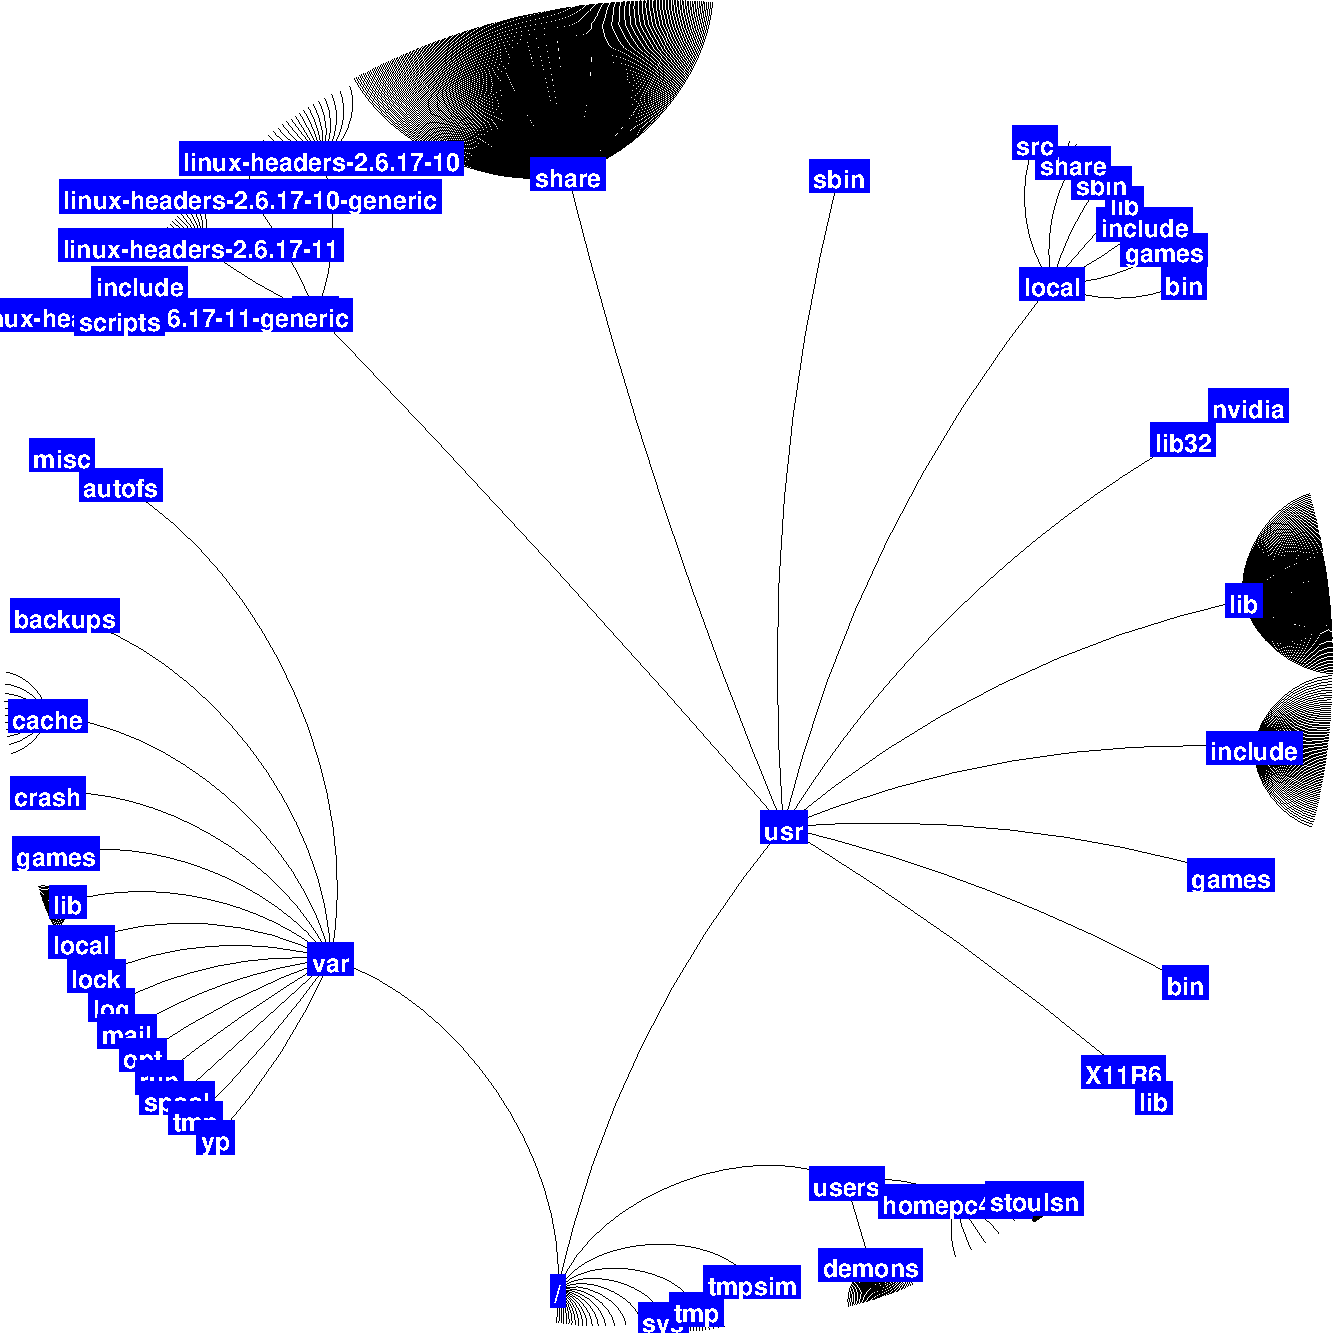
\includegraphics[scale=0.3]{images/htree.pdf}   
    \end{center}
  \end{figure}
\end{frame}

\begin{frame}
  \frametitle{Plan}
  \begin{itemize}
  \item La g�om�trie hyperbolique
  \item La visualisation de graphes en g�om�trie hyperbolique
  \item D�monstration du programme
  \end{itemize}
\end{frame}


\begin{frame}
  \frametitle{Historique}
  \begin{itemize}
  \item G�om�trie euclidienne et le  $V^e$ postulat
    \begin{quote}
      ``�tant donn�s une droite $D$ et un point M, il n'existe qu'une seule
      droite passant par $M$ et qui soit parall�le � $D$.''
    \end{quote}
  \item Th�ories de Bolyai et Lobatchevsky
    \bigskip
    \begin{center}
           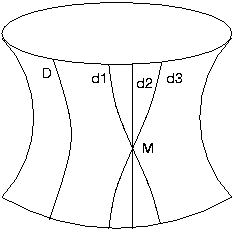
\includegraphics[height=2.5cm]{images/parallels.png}
    \end{center}
  \end{itemize}
\end{frame}

\begin{frame}
  \frametitle{Mod�le de Poincar�}

  Transposition du plan euclidien dans le disque unit�

  \begin{center}
        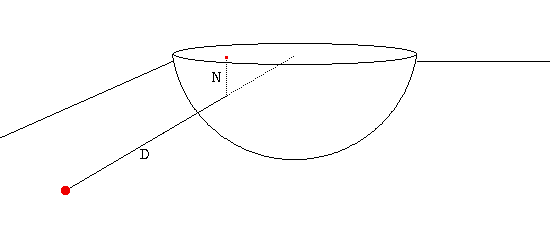
\includegraphics[scale=0.5]{images/lentille1.png}   
  \end{center}
\end{frame}

\begin{frame}
  \frametitle{Disque de Poincar�}
  Droites euclidiennes sont des arcs de cercle
  \begin{center}
        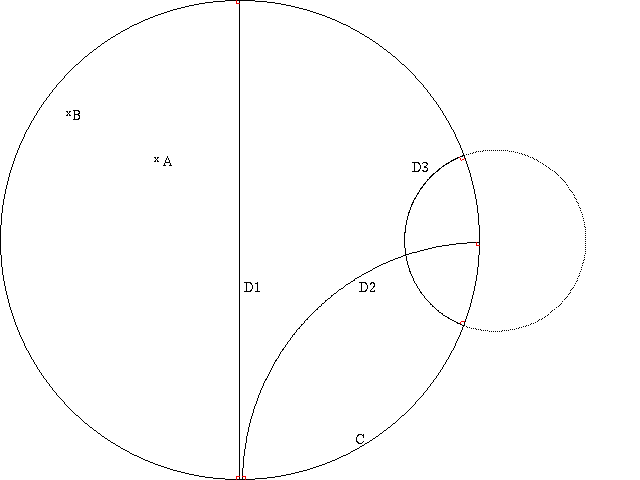
\includegraphics[scale=0.3]{images/perpendiculaire.png}   
  \end{center}
  Adaptation de la tortue LOGO du plan euclidien au disque de Poincar�  
\end{frame}

\begin{frame}
  \frametitle{Application � la visualisation de graphes}
R�partition du plan entre les successeurs de la racine
  \begin{center}
    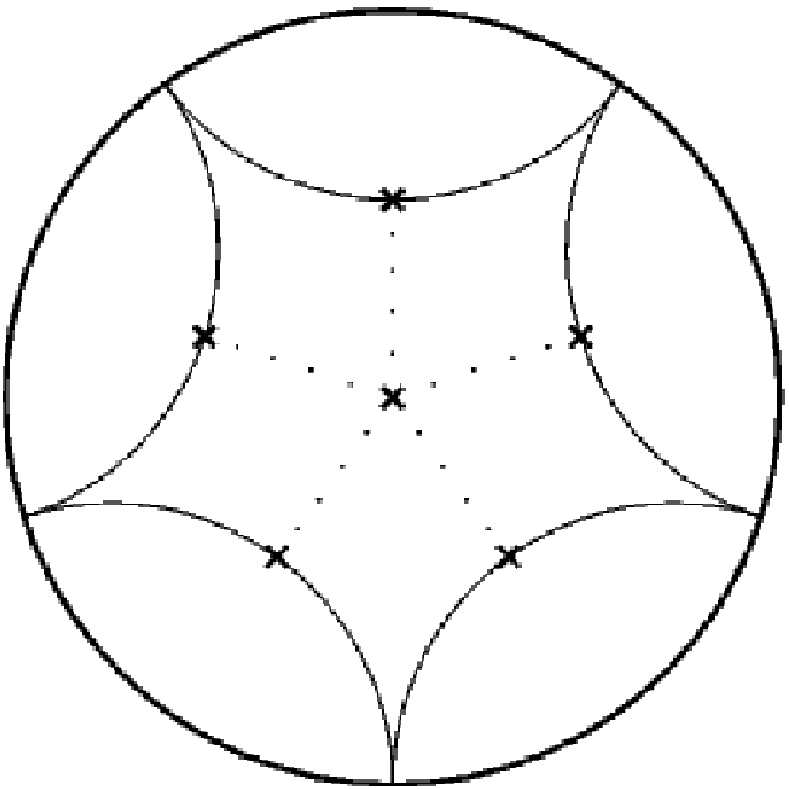
\includegraphics[scale=0.3027]{images/dictateurs.jpg}   
  \end{center}
\end{frame}

\begin{frame}
  \frametitle{Application � la visualisation de graphes}
R�partition d'un demi-plan entre les successeurs d'un n\oe ud
  \begin{center}
    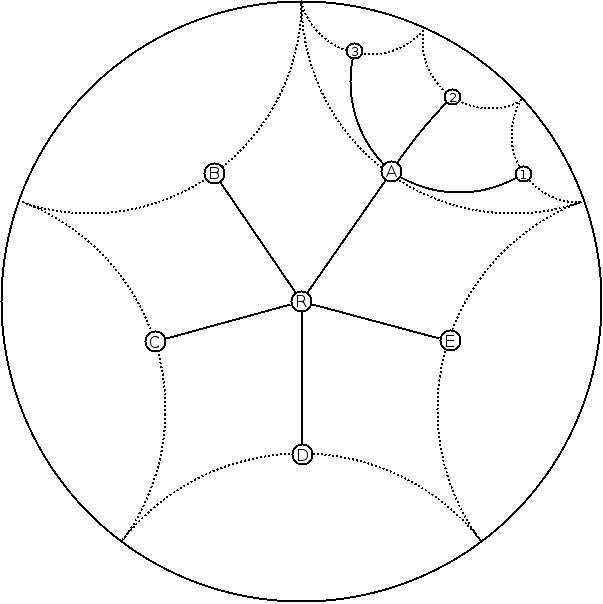
\includegraphics[scale=0.3]{images/dictateursniv2.jpg}   
  \end{center}
\end{frame}

\begin{frame}
  \frametitle{Application � la visualisation de graphes}
Ar�tes s'affranchissant des fronti�res entre demi-plans \smallskip
  \begin{center}
    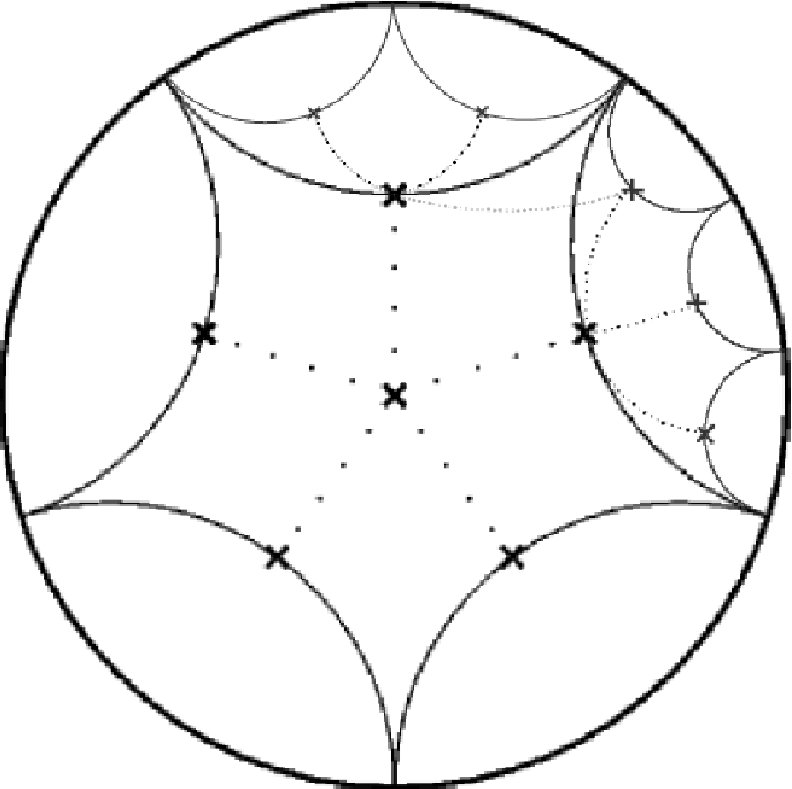
\includegraphics[scale=0.3]{images/intern-edge.jpg}   
  \end{center}
\end{frame}

\begin{frame}
  \frametitle{Application � la visualisation de graphes}
Deux parcours possibles : en profondeur (Dfs) et en largeur (Bfs)
  \begin{center}
   \begin{minipage}{0.49\linewidth}
    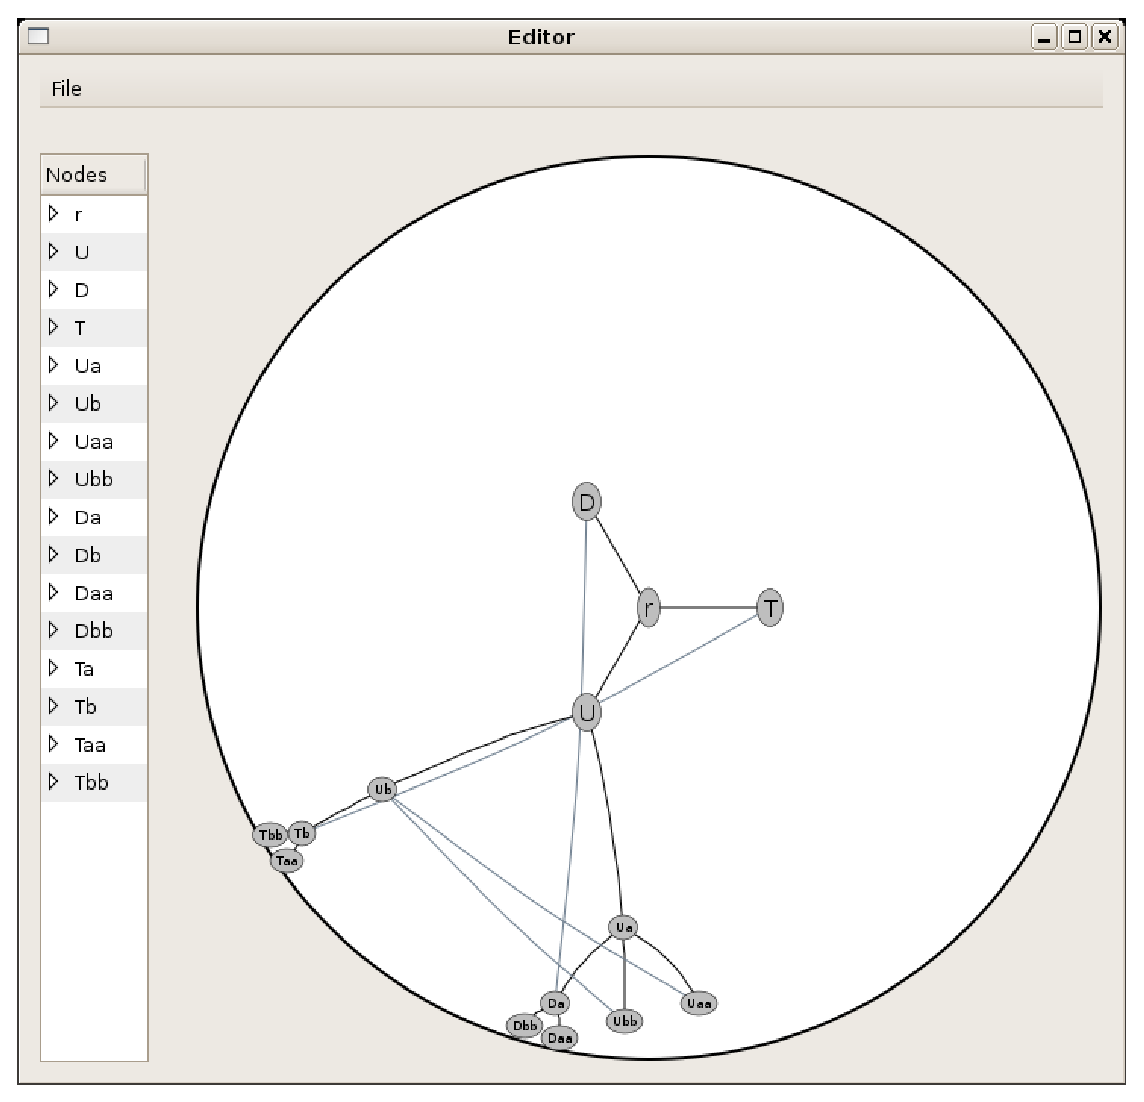
\includegraphics[scale=0.30]{images/parcours_dfs.eps} 
  \end{minipage}
  \begin{minipage}{0.49\linewidth}
    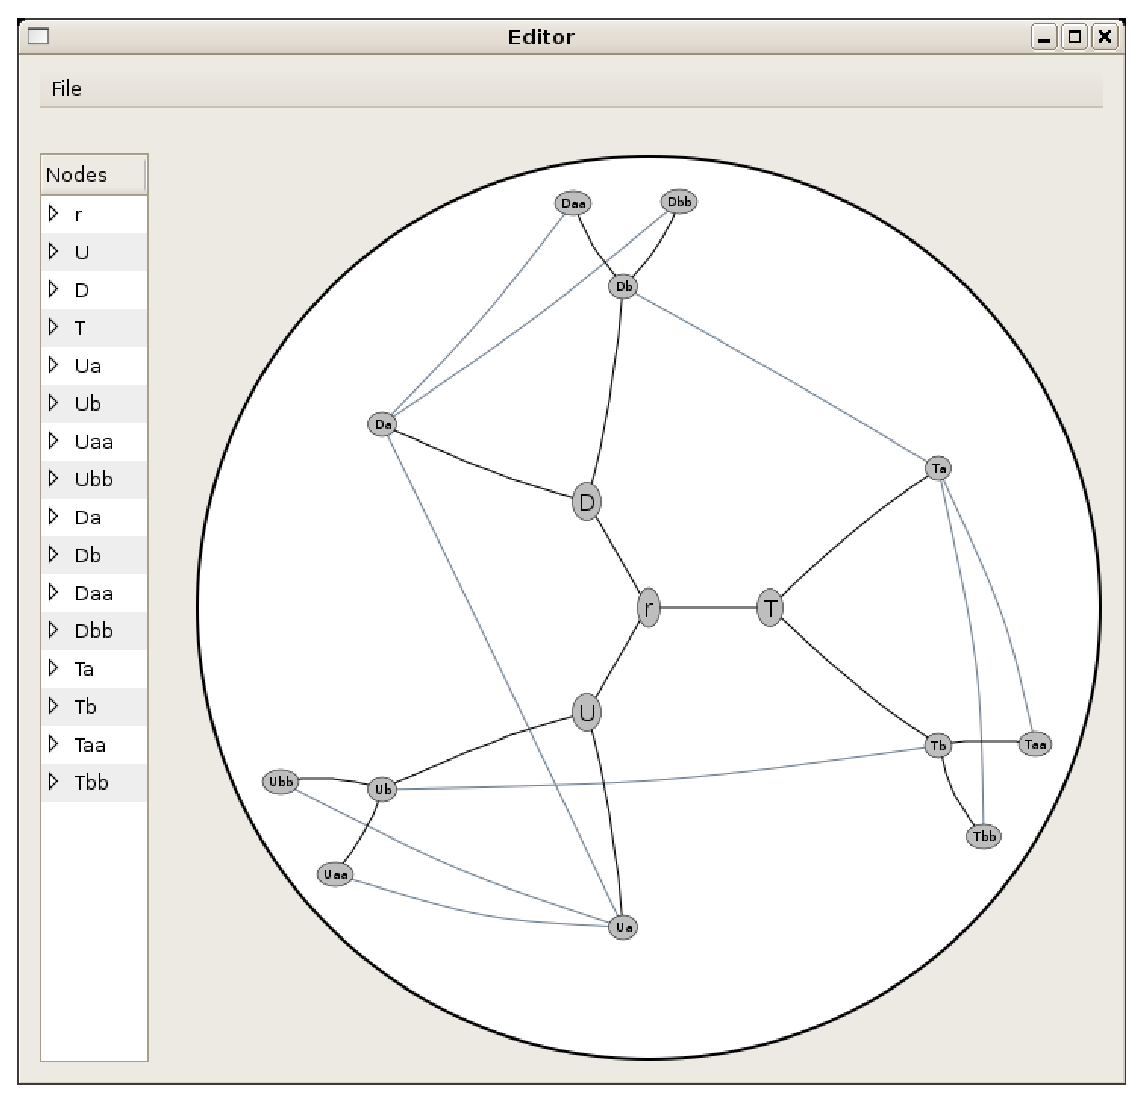
\includegraphics[scale=0.30]{images/parcours_bfs.eps}
  \end{minipage}

  \end{center}
\end{frame}

% 2 autres transparents expliquant les solutions : le parcours / l'ordonnancement des successeurs

% 1 transparent sur la r�alisation en Ocaml

\begin{frame}
  \begin{center}
    D�monstration
  \end{center}
\end{frame}

\begin{frame}
  % extensions possibles
\end{frame}

\end{document}

%%% Local Variables: 
%%% mode: latex
%%% TeX-master: t
%%% End: 
